\begin{tikzpicture}[every node/.style={inner sep=0pt}]
\foreach \coord/\name in {{(0,0)}/first,{(2.7,0.3)}/second,{(5.4,0)}/third} {
	\node (\name-cpu) at \coord {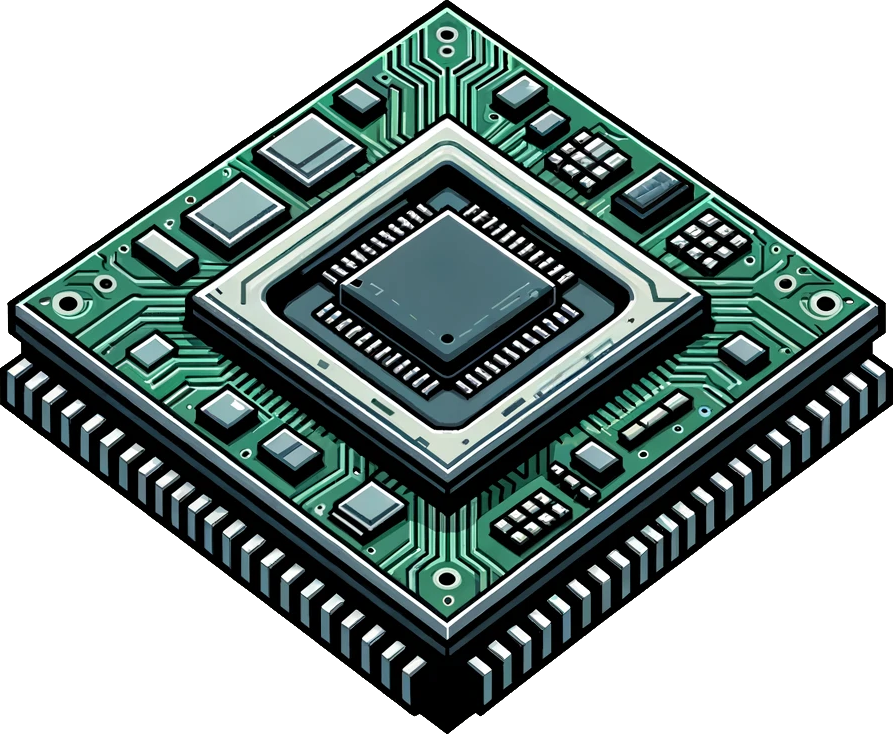
\includegraphics[scale=0.065]{images/cpu}};
    \fill[white] ($(\name-cpu)+(4pt, -10pt)$) -- ($(\name-cpu)+(4pt, 19pt)$) -- ($(\name-cpu)+(20pt, 19pt)$) -- ($(\name-cpu)+(28pt, 13pt)$) -- ($(\name-cpu)+(28pt, -10pt)$) -- cycle;
	\node[anchor=north] at ($(\name-cpu)+(16pt, 20pt)$) {{\fontsize{30}{30}\selectfont\faFileTextO}};
}
\node[below=.3ex] at (first-cpu.south) { used };
\node[below=.3ex] at (second-cpu.south) { used };
\node[below=.3ex] at (third-cpu.south) { used };
\end{tikzpicture}%